\documentclass[12pt,titlepage]{article}
\usepackage[margin=1.25in]{geometry}
\usepackage{graphicx,amsmath,minted,enumitem}

%% Variables definition
\newcommand{\vSubject}{Advanced Database}
\newcommand{\vSubtitle}{Jobsheet 10}
\newcommand{\vName}{Dicha Zelianivan Arkana}
\newcommand{\vNIM}{2241720002}
\newcommand{\vClass}{2i}
\newcommand{\vDepartment}{Information Technology}
\newcommand{\vStudyProgram}{D4 Informatics Engineering}

%% [START] Tikz related stuff
\usepackage{tikz}
\usetikzlibrary{svg.path,calc,shapes.geometric,shapes.misc}
\tikzstyle{terminator} = [rectangle, draw, text centered, rounded corners = 1em, minimum height=2em]
\tikzstyle{preparation} = [chamfered rectangle, chamfered rectangle sep=0.75em, draw, text centered, minimum height = 2em]
\tikzstyle{process} = [rectangle, draw, text centered, minimum height=2em]
\tikzstyle{decision} = [diamond, aspect=2, draw, text centered, minimum height=2em]
\tikzstyle{data}=[trapezium, draw, text centered, trapezium left angle=60, trapezium right angle=120, minimum height=2em]
\tikzstyle{connector} = [line width=0.25mm,->]
%% [END] Tikz related stuff

%% [START] Fancy header related stuff
\usepackage{fancyhdr}
\pagestyle{fancy}
\setlength{\headheight}{15pt} % compensate fancyhdr style
\fancyhead{}
\fancyfoot{}
\fancyfoot[L]{\thepage}
\fancyfoot[R]{\textit{\vSubject - \vSubtitle}}
\renewcommand{\footrulewidth}{0.4pt}% default is 0pt, overline for footer
%% [END] Fancy header related stuff

%% [START] Custom tabular command related stuff
\usepackage{tabularx}
\newcommand{\details}[2]{
    #1 & #2  \\
}
%% [END] Custom tabular command related stuff

%% [START] Figure related stuff
\newcommand{\image}[3][1]{
    \begin{figure}[h]
        \centering
        \includegraphics[#1]{#2}
        \caption{#3}
        \label{#3}
    \end{figure}
}
%% [END] Figure related stuff

\begin{document}
\begin{titlepage}
    \centering
    \vfill
    {\bfseries\LARGE
        \vSubject\\
        \vskip0.25cm
        \vSubtitle
    }
    \vfill
    
\includegraphics[width=6cm]{images/polinema-logo.png}
    \vfill
    {
        \textbf{Name}\\
        \vName\\
        \vskip0.5cm
        \textbf{NIM}\\
        \vNIM\\
        \vskip0.5cm
        \textbf{Class}\\
        \vClass\\
        \vskip0.5cm
        \textbf{Department}\\
        \vDepartment\\
        \vskip0.5cm
        \textbf{Study Program}\\
        \vStudyProgram
    }
\end{titlepage}

\section{Practicum}
\begin{enumerate}
    \item {
        Buka prompt jalankan perintah berikut ini :\\
        \texttt{C$\backslash$>Program Files$\backslash$xampp$\backslash$mysql$\backslash$bin>mysql $-$u root $-$p (enter)}
        \begin{figure}[h]
            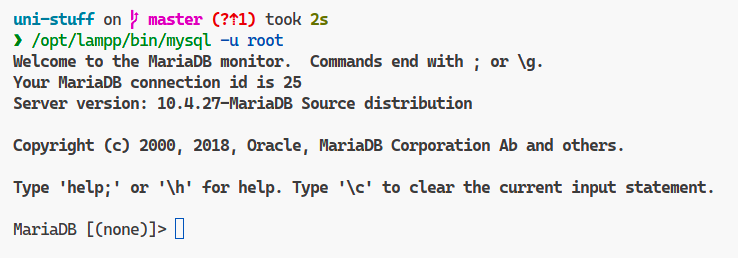
\includegraphics[width=.8\textwidth]{./images/practicum-1.png}
        \end{figure}
    }
    \item {
        Buatlah sebuah database dengan nama \texttt{db\_polinema}\\
        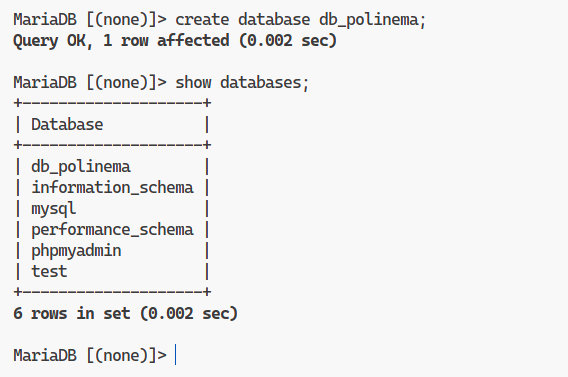
\includegraphics[width=.8\textwidth]{./images/practicum-2.png}
    }
    \item {
        Tabel \texttt{prodi}\\
        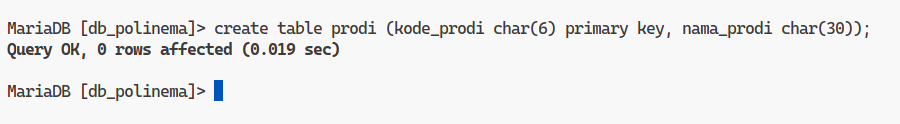
\includegraphics[width=.8\textwidth]{./images/practicum-3.png}
    }
    \item {
        Tabel \texttt{mahasiswa}\\
        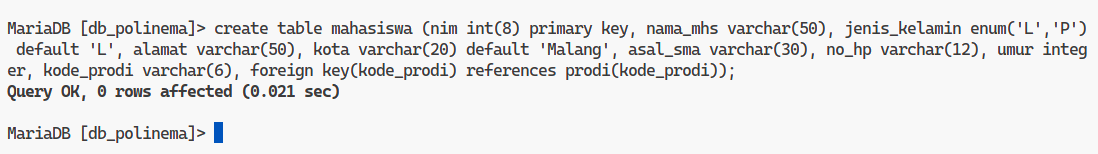
\includegraphics[width=.8\textwidth]{./images/practicum-4.png}
    }
    \item {
        Tabel \texttt{mata\_kuliah}\\
        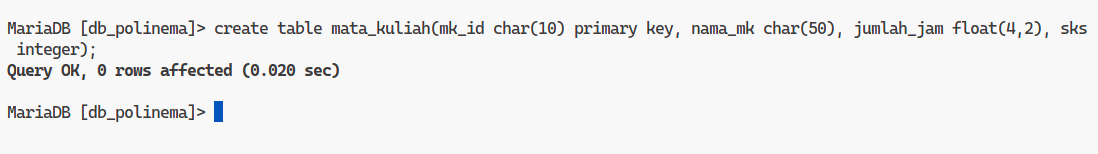
\includegraphics[width=.8\textwidth]{./images/practicum-5.png}
    }
    \item {
        Tabel \texttt{ruang}\\
        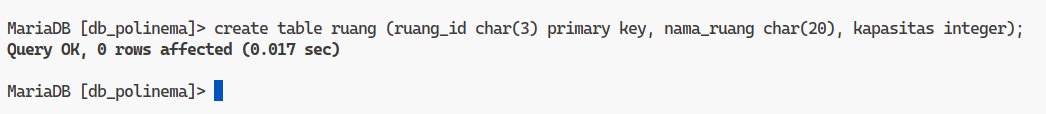
\includegraphics[width=.8\textwidth]{./images/practicum-6.png}
    }
    \item {
        Tabel \texttt{dosen}\\
        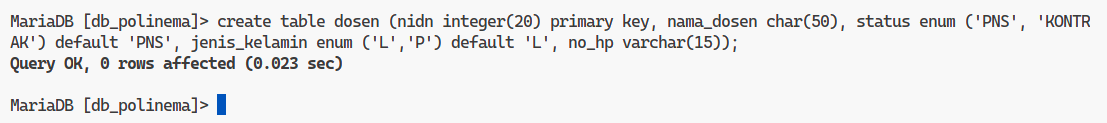
\includegraphics[width=.8\textwidth]{./images/practicum-7.png}
    }
    \item {
        Tambahkan sebuah kolom \texttt{agama (varchar(10))} pada tabel \texttt{mahasiswa} sebagai kolom terakhir\\
        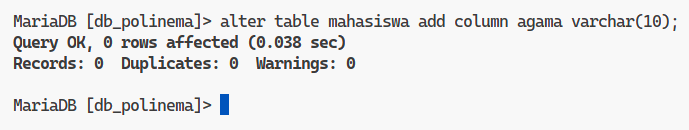
\includegraphics[width=.8\textwidth]{./images/practicum-8.png}
    }
    \item {
        Tambahkan kolom \texttt{alamat(varchar(50))} pada tabel \texttt{dosen} sebagai kolom terakhir\\
        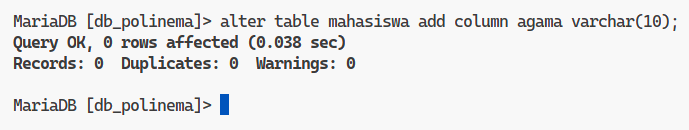
\includegraphics[width=.8\textwidth]{./images/practicum-8.png}
    }
    \item {
        Lakukan insert data ke dalam tabel-tabel yang ada pada pada database\\
        \texttt{db\_polinema} sesuai dengan field, tipe data dan panjang datanya\\
        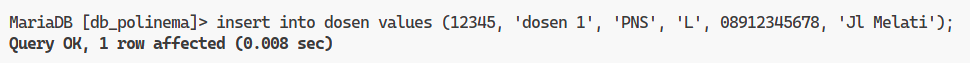
\includegraphics[width=.8\textwidth]{./images/practicum-10a.png}\\
        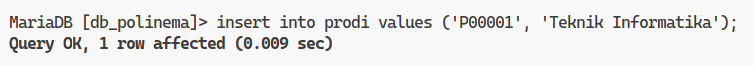
\includegraphics[width=.8\textwidth]{./images/practicum-10b.png}\\
        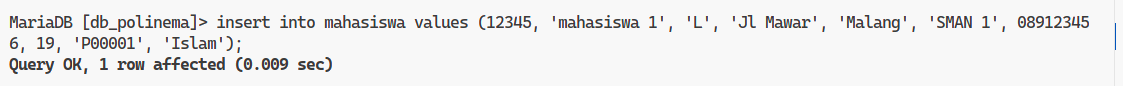
\includegraphics[width=.8\textwidth]{./images/practicum-10c.png}\\
        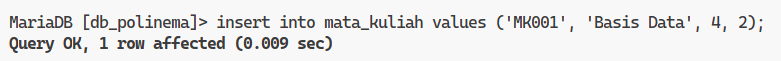
\includegraphics[width=.8\textwidth]{./images/practicum-10d.png}\\
        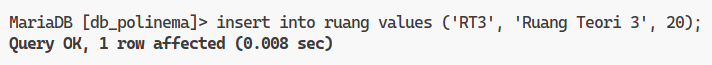
\includegraphics[width=.8\textwidth]{./images/practicum-10e.png}\\
    }
    \pagebreak
    \item {
        Tampilkan semua tabel yang ada didalam database \texttt{db\_polinema}\\
        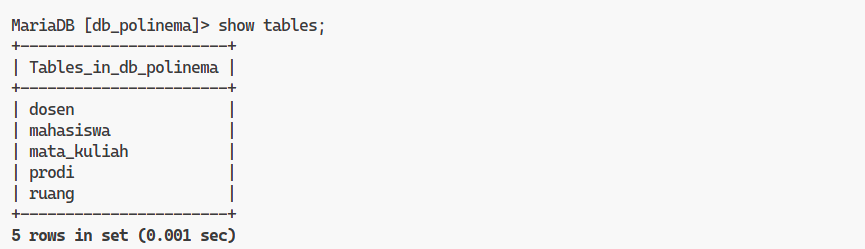
\includegraphics[width=.8\textwidth]{./images/practicum-11.png}
    }
    \item {
        Tampilkan semua isi tabel yang ada didalam tabel \texttt{mahasiswa}\\
        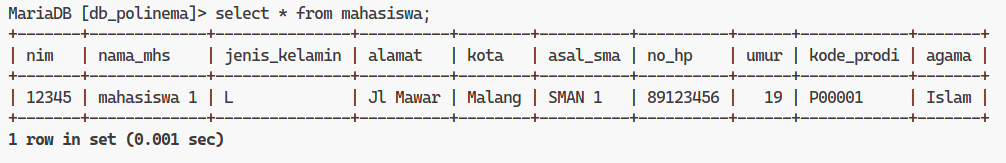
\includegraphics[width=.8\textwidth]{./images/practicum-12.png}
    }
    \item {
        Tampilkan struktur(metadata) tabel \texttt{mahasiswa}\\
        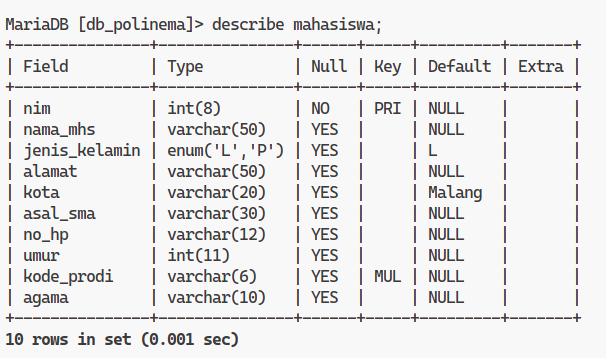
\includegraphics[width=.8\textwidth]{./images/practicum-13.png}
    }
    \item {
        Hilangkan kolom \texttt{asal\_sma} yang terdapat didalam tabel \texttt{mahasiswa}\\
        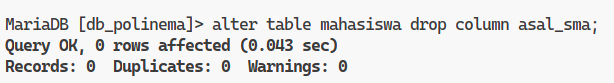
\includegraphics[width=.8\textwidth]{./images/practicum-14.png}
    }
\end{enumerate}
\pagebreak

\section{Tugas}
\begin{enumerate}
    \item {
        Buatlah basis data Akademik dengan data sebagai berikut

        \begin{figure}[h]
            \centering
            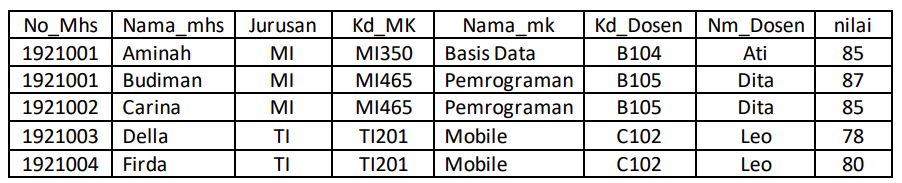
\includegraphics[width=\textwidth]{./images/task-1.png}
        \end{figure}

        \begin{enumerate}[label=\alph*.]
            \item {
                \begin{minted}[fontsize=\small,autogobble]{sql}
                    CREATE TABLE Mahasiswa (
                        No_Mhs   CHAR(7)     NOT NULL PRIMARY KEY,
                        Nama_mhs VARCHAR(50) NOT NULL
                    );

                    CREATE TABLE Mata_Kuliah (
                        Kd_MK    CHAR(5)     NOT NULL PRIMARY KEY,
                        Nama_MK  VARCHAR(50) NOT NULL
                    );

                    CREATE TABLE Nilai (
                        No_Mhs   CHAR(7)     NOT NULL,
                        Kode_MK  CHAR(5)     NOT NULL
                    );

                    ALTER TABLE Mahasiswa ADD COLUMN Jurusan VARCHAR(50);
                \end{minted}
            }
            \item {
                \begin{minted}[fontsize=\small,autogobble]{sql}
                    ALTER TABLE Mata_Kuliah ADD COLUMN Kd_Dosen VARCHAR(50);
                \end{minted}
            }
            \item {
                \begin{minted}[fontsize=\small,autogobble]{sql}
                    ALTER TABLE Nilai ADD COLUMN Nilai FLOAT(4,2);
                    ALTER TABLE Nilai ADD CONSTRAINT `fk_nilai_mhs` FOREIGN KEY (No_Mhs) REFERENCES Mahasiswa(No_Mhs);
                    ALTER TABLE Nilai ADD CONSTRAINT `fk_nilai_mk` FOREIGN KEY (Kode_MK) REFERENCES Mata_Kuliah(Kd_MK);
                \end{minted}
            }
            \item {
                \begin{minted}[fontsize=\small,autogobble]{sql}
                    CREATE TABLE Dosen (
                        Kd_Dosen CHAR(5)       NOT NULL PRIMARY KEY,
                        Nama_Dosen VARCHAR(50) NOT NULL
                    );
                \end{minted}
            }
            \item {
                \begin{minted}[fontsize=\small,autogobble]{sql}
                    INSERT INTO Mahasiswa
                    VALUES ('1921000', 'Aminah', 'MI'),
                           ('1921001', 'Budiman', 'MI'),
                           ('1921002', 'Carina', 'MI'),
                           ('1921003', 'Della', 'TI'),
                           ('1921004', 'Firda', 'TI');

                    INSERT INTO Dosen
                    VALUES ('B104', 'Ati'),
                           ('B105', 'Dita'),
                           ('C102', 'Leo');

                    INSERT INTO Mata_Kuliah
                    VALUES ('MI350', 'Basis Data', 'B104'),
                           ('MI465', 'Pemrograman', 'B105'),
                           ('TI201', 'Mobile', 'C102');

                    INSERT INTO Nilai
                    VALUES ('1921000', 'MI350', 85),
                           ('1921001', 'MI465', 87),
                           ('1921002', 'MI465', 85),
                           ('1921003', 'TI201', 78),
                           ('1921004', 'TI201', 80);
                \end{minted}
            }
            \item {
                \begin{minted}[fontsize=\small,autogobble]{sql}
                    SELECT
                        Mahasiswa.No_Mhs as 'No_Mhs',
                        Mahasiswa.Nama_Mhs as 'Nama_Mhs',
                        Mahasiswa.Jurusan as 'Jurusan',
                        Mata_Kuliah.Kd_MK as 'Kd_MK',
                        Mata_Kuliah.Nama_MK as 'Nama_MK',
                        Dosen.Kd_Dosen as 'Kd_Dosen',
                        Dosen.Nama_Dosen as 'Nama_Dosen',
                        Nilai.Nilai as 'Nilai'
                    FROM Mahasiswa
                    JOIN Nilai ON Mahasiswa.No_Mhs = Nilai.No_Mhs
                    JOIN Mata_Kuliah ON Nilai.Kode_MK = Mata_Kuliah.Kd_MK
                    JOIN Dosen ON Mata_Kuliah.Kd_Dosen = Dosen.Kd_Dosen;
                \end{minted}
                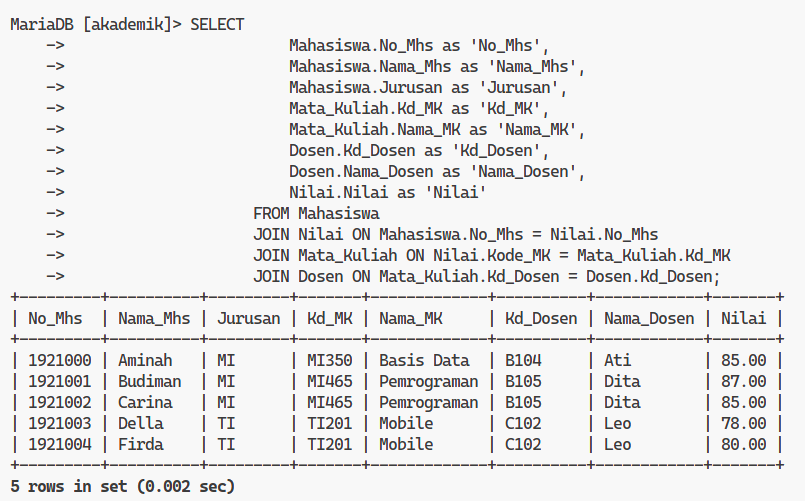
\includegraphics[width=.6\textwidth]{./images/query-all.png}
            }
        \end{enumerate}
    }
    \pagebreak
    \item {
        Buatlah basis data Pegawai yang terdiri dari tabel sebagai berikut:
        \begin{figure}[h]
            \centering
            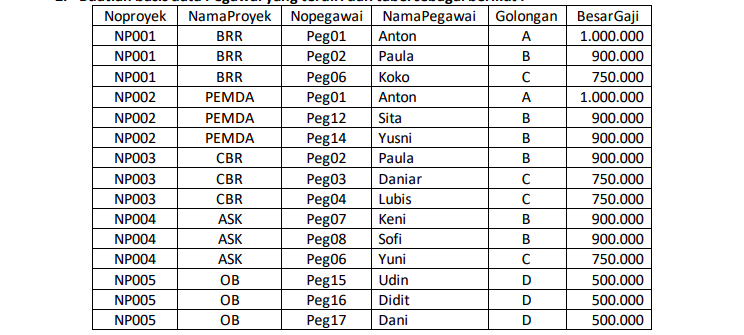
\includegraphics[width=\textwidth]{./images/task-2.png}
        \end{figure}

        \begin{enumerate}[label=\alph*.]
            \item {
                \begin{minted}[fontsize=\small,autogobble]{sql}
                    CREATE TABLE Pegawai (
                        Nopegawai     CHAR(5)     NOT NULL PRIMARY KEY,
                        NamaPegawai   VARCHAR(50) NOT NULL
                    );

                    CREATE TABLE Golongan (
                        Golongan CHAR(1)     NOT NULL PRIMARY KEY
                    );

                    CREATE TABLE Proyek (
                        Noproyek CHAR(5)     NOT NULL PRIMARY KEY
                    );

                    CREATE TABLE Proyekpegawai (
                        Noproyek CHAR(5)     NOT NULL
                    );
                \end{minted}
            }
            \item {
                \begin{minted}[fontsize=\small,autogobble]{sql}
                    ALTER TABLE Pegawai ADD COLUMN Golongan CHAR(1);
                \end{minted}
            }
            \item {
                \begin{minted}[fontsize=\small,autogobble]{sql}
                    ALTER TABLE Golongan ADD COLUMN BesarGaji INT(10);
                \end{minted}
            }
            \item {
                \begin{minted}[fontsize=\small,autogobble]{sql}
                    ALTER TABLE Proyek ADD COLUMN NamaProyek VARCHAR(50);
                \end{minted}
            }
            \item {
                \begin{minted}[fontsize=\small,autogobble]{sql}
                    ALTER TABLE Proyekpegawai ADD COLUMN Nopegawai CHAR(5);
                    ALTER TABLE Proyekpegawai ADD CONSTRAINT `fk_proyekpegawai_proyek` FOREIGN KEY (Noproyek) REFERENCES Proyek(Noproyek);
                    ALTER TABLE Proyekpegawai ADD CONSTRAINT `fk_proyekpegawai_pegawai` FOREIGN KEY (Nopegawai) REFERENCES Pegawai(Nopegawai);
                \end{minted}
            }
            \item {
                \begin{minted}[fontsize=\small,autogobble]{sql}
                    INSERT INTO Golongan
                    VALUES ('A', 1000000),
                           ('B',  900000),
                           ('C',  750000),
                           ('D',  500000);

                    INSERT INTO Pegawai
                    VALUES ('Peg01', 'Anton', 'A'),
                           ('Peg02', 'Paulia', 'B'),
                           ('Peg03', 'Daniar', 'C'),
                           ('Peg04', 'Lubis', 'C'),
                           ('Peg06', 'Koko', 'C'),
                           ('Peg07', 'Keni', 'B'),
                           ('Peg08', 'Sofi', 'B'),
                           ('Peg12', 'Sita', 'B'),
                           ('Peg14', 'Yusni', 'B'),
                           ('Peg15', 'Udin', 'D'),
                           ('Peg16', 'Didit', 'D'),
                           ('Peg17', 'Dani', 'D');

                    INSERT INTO Proyek
                    VALUES ('NP001', 'BRR'),
                           ('NP002', 'PEMDA'),
                           ('NP003', 'CBR'),
                           ('NP004', 'ASK'),
                           ('NP005', 'OB');

                    INSERT INTO Proyekpegawai
                    VALUES ('NP001', 'Peg01'),
                           ('NP001', 'Peg02'),
                           ('NP001', 'Peg06'),
                           ('NP002', 'Peg01'),
                           ('NP002', 'Peg12'),
                           ('NP002', 'Peg14'),
                           ('NP003', 'Peg02'),
                           ('NP003', 'Peg03'),
                           ('NP003', 'Peg04'),
                           ('NP004', 'Peg07'),
                           ('NP004', 'Peg08'),
                           ('NP004', 'Peg06'),
                           ('NP005', 'Peg15'),
                           ('NP005', 'Peg16'),
                           ('NP005', 'Peg17');
                \end{minted}
            }
            \item {
                \begin{minted}[fontsize=\small,autogobble]{sql}
                    SELECT
                        Proyek.Noproyek as 'Noproyek',
                        Proyek.NamaProyek as 'NamaProyek',
                        Pegawai.Nopegawai as 'Nopegawai',
                        Pegawai.NamaPegawai as 'NamaPegawai',
                        Golongan.Golongan as 'Golongan',
                        Golongan.BesarGaji as 'BesarGaji'
                    FROM Pegawai
                    JOIN Golongan ON Pegawai.Golongan = Golongan.Golongan
                    JOIN Proyekpegawai ON Pegawai.Nopegawai = Proyekpegawai.Nopegawai
                    JOIN Proyek ON Proyekpegawai.Noproyek = Proyek.Noproyek;
                \end{minted}
                \begin{center}
                    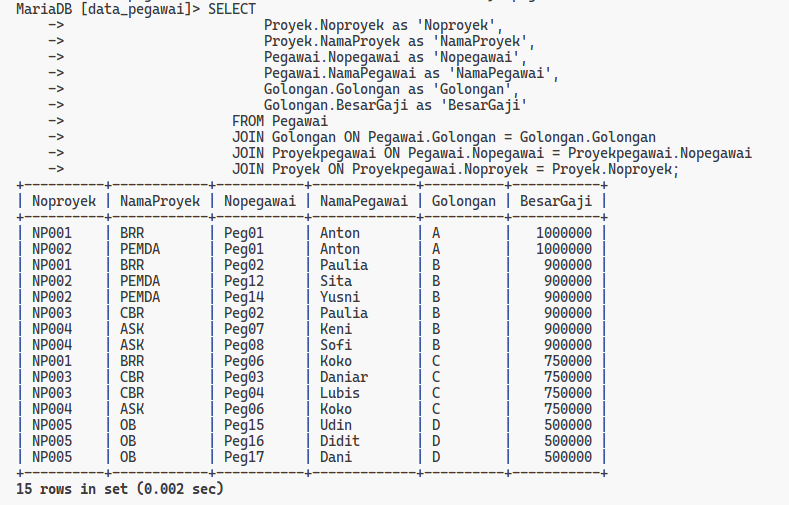
\includegraphics[width=.8\textwidth]{./images/query-all-2.png}
                \end{center}
            }
        \end{enumerate}
    }
\end{enumerate}

\end{document}

